% $Header: /u/gcmpack/manual/s_under_dvlp/text/time_stepping_dvlp.tex,v 1.3 2010/08/25 03:00:54 jmc Exp $
% $Name:  $

\section{Other Time-stepping Options}
%\begin{rawhtml}
%<!-- CMIREDIR:dvlp-time-stepping: -->
%\end{rawhtml}

\subsection{Adams-Bashforth III}

\begin{figure}[ht]
\begin{center}
\resizebox{10cm}{!}{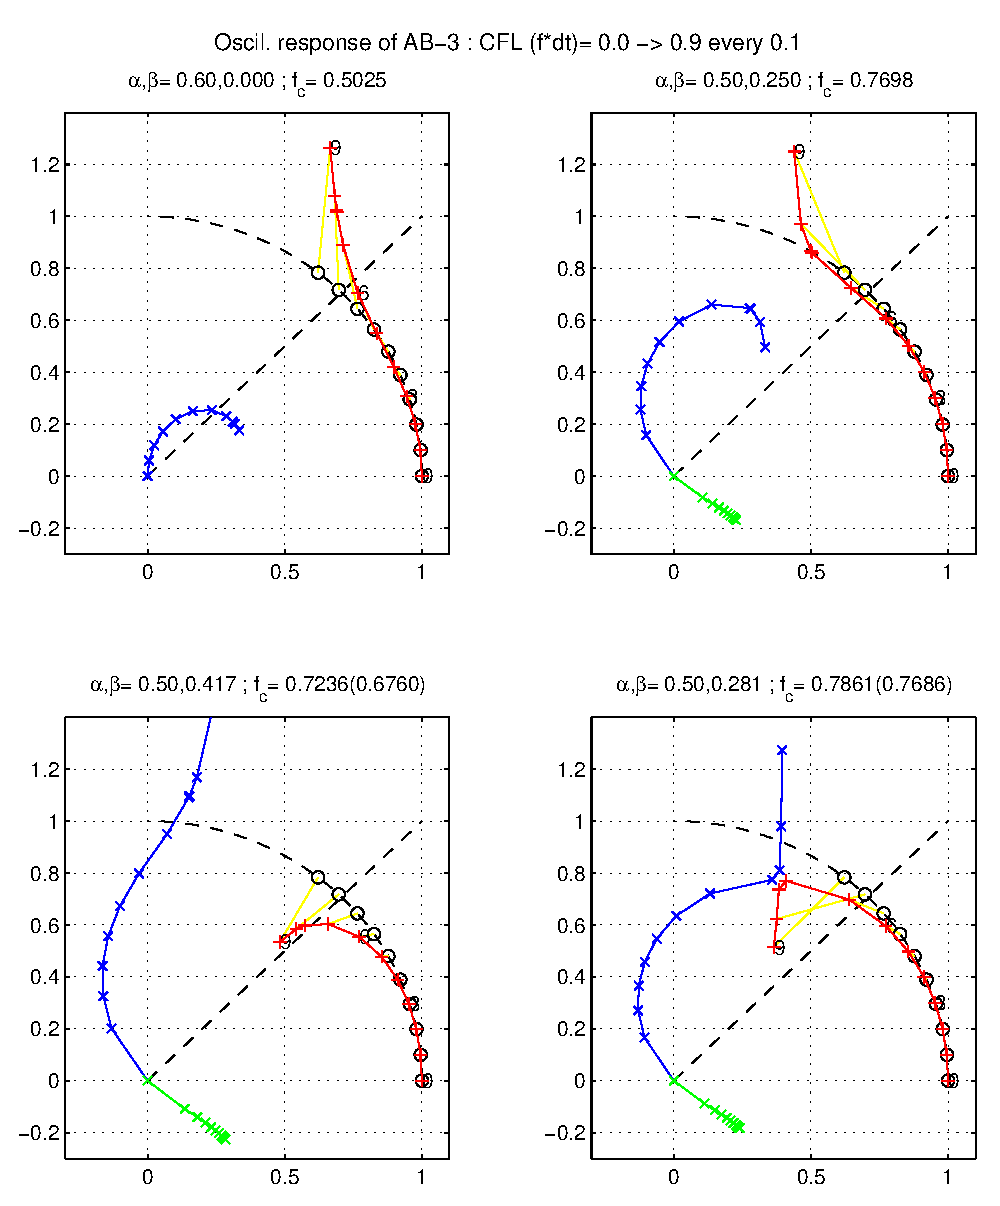
\includegraphics{under_dvlp/stab_AB3_oscil.eps}}
\end{center}
\caption{
Comparison of the oscillatory response of Adams-Bashforth scheme.
}
\label{fig:ab_oscill_response}
\end{figure}

The third-order Adams-Bashforth time stepping (AB-3) provides
several advantages (see, e.g., \cite{durr:91}) compared to
the default quasi-second order Adams-Bashforth (AB-2):
\begin{itemize}
\item higher accuracy;
\item stable with a longer time-step;
\item no additional computation (just requires the storage of one additional 
 time level).
\end{itemize}

The $3^{rd}$ order Adams-Bashforth can be used to 
extrapolate forward in time the tendency
(replacing equation \ref{eq:adams-bashforth2}) 
which writes:
\begin{equation}
G_\tau^{(n+1/2)} = ( 1 + \alpha_{AB} + \beta_{AB}) G_\tau^n
- ( \alpha_{AB} + 2 \beta_{AB}) G_\tau^{n-1}
+ \beta_{AB} G_\tau^{n-2}
\label{eq:adams-bashforth3}
\end{equation}
The 3rd order AB is obtained 
with $(\alpha_{AB},\,\beta_{AB}) = (1/2,\,5/12)$.
Note that selecting 
$(\alpha_{AB},\,\beta_{AB}) = (1/2+\epsilon_{AB},\,0)$
one recovers the quasi-2nd order AB.
%as illustrated on fig.\ref{fig:adams-bashforth-respons}.

The AB-3 time stepping improves the stability limit
for an oscillatory problem like advection or Coriolis. 
As seen from Fig.\ref{fig:ab_oscill_response},
it remains stable up to a CFL of 0.72, 
compared to only 0.50 with AB-2 and $\epsilon_{AB} = 0.1$.
%
It is interesting to note that the stability limit can be further
extended up to a CFL of 0.786 for an oscillatory problem 
(see fig.\ref{fig:ab_oscill_response})
using $(\alpha_{AB},\,\beta_{AB}) = (0.5,\,0.2811)$
but then the scheme is only 2nd order accurate.

\begin{figure}[ht]
\begin{center}
\resizebox{10cm}{!}{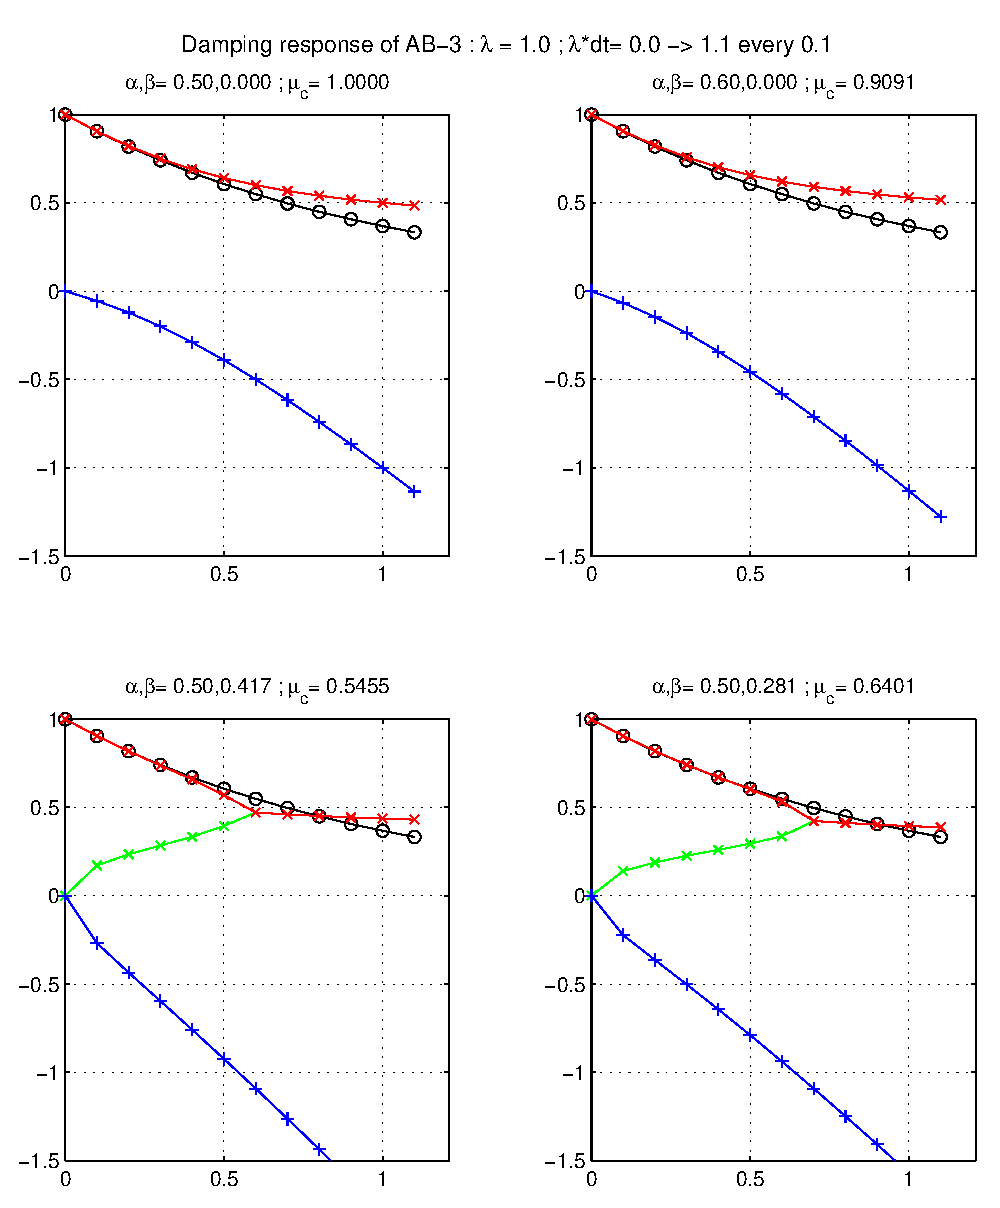
\includegraphics{under_dvlp/stab_AB3_dampR.eps}}
\end{center}
\caption{
Comparison of the damping (diffusion like) response of Adams-Bashforth schemes.
}
\label{fig:ab_damp_response}
\end{figure}

However, the behavior of the AB-3 for a damping problem (like diffusion)
is less favorable, since the stability limit is reduced to 
0.54 only (and 0.64 with $\beta_{AB} = 0.2811$) compared to 1. (and 0.9 
with $\epsilon_{AB} = 0.1$) with the AB-2 (see fig.\ref{fig:ab_damp_response}).

A way to enable the use of a longer time step is
to keep the dissipation terms outside the AB extrapolation
(setting {\em momDissip\_In\_AB=.FALSE.} in main parameter file 
"\texttt{data}", namelist {\em PARM03}),
thus returning to a simple forward time-stepping for dissipation,
and to use AB-3 only for advection and Coriolis terms.

The AB-3 time stepping is activated by defining the option
{\em \#define ALLOW\_ADAMSBASHFORTH\_3}
in "\texttt{CPP\_OPTIONS.h}".
The parameters $\alpha_{AB},\beta_{AB}$ can be set from the
main parameter file "\texttt{data}" (namelist {\em PARM03}) and their 
default value corresponds to the 3rd order Adams-Bashforth.
A simple example is provided in "\texttt{verification/advect\_xy/input.ab3\_c4}".

The AB-3 is not yet available for 
the vertical momentum equation (Non-Hydrostatic) 
neither for passive tracers.

\subsection{Time-extrapolation of tracer (rather than tendency)}
 (to be continued ...)
